\chapter{同伦}

\section{同伦}


\begin{definition}{同伦}
    设$X,Y$是拓扑空间，$f,g:X\to Y$是两个连续映射，如果存在一个连续映射$H:X\times[0,1]\to Y$，使得$H(x,0)=f(x),H(x,1)=g(x)$，则称$f$和$g$是\textbf{同伦的}，记作$f\simeq g$，映射$H$称为从$f$到$g$的\textbf{同伦}，记作$H:f\simeq g$.
\end{definition}

\begin{figure}[h]
    \centering
    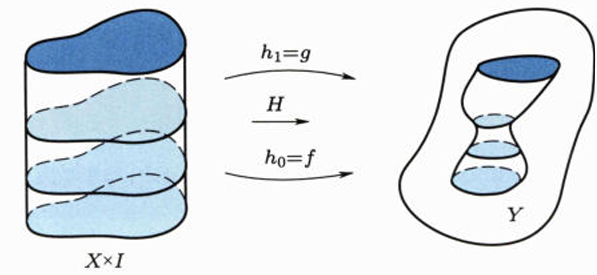
\includegraphics[width=0.6\textwidth]{fig/10.1.png}
    \caption{同伦示意图}
\end{figure}
如果固定$t$，可以定义函数$\setjot[-6]\begin{aligned}[t]
    h_t:X&\to Y \\
    x&\mapsto H(x,t)
\end{aligned} $，如果固定$x$，则$\setjot[-6]\begin{aligned}[t]
    a_x:[0,1]&\to Y \\
    t&\mapsto H(x,t)
\end{aligned}$是一条道路.

\begin{instance}
    设$X$是一个拓扑空间，$Y$是$\mb{E}^n$的凸子空间，任取$f,g:X\to Y$，则$f\simeq g$.\par
    可以构造$\setjot[-6]\begin{aligned}[t]
        H:X\times [0,1]&\to Y \\
        (x,t) &\mapsto (1-t)f(x)+tg(x)
     \end{aligned}$.则$H(x,0)=f(x),H(x,1)=g(x)$.\par
     这种同伦称为\bluebf{直线同伦}.
\end{instance}

\begin{instance}
    设$f,g:X\to S^n$，且$\forall\, x\in X$，$f(x)+g(x)\neq 0$，则$f\simeq g$.\par
    构造$\setjot[-6]\begin{aligned}[t]
        H:X\times [0,1]&\to S^n \\
        (x,t) &\mapsto \frac{(1-t)f(x)+tg(x)}{\|(1-t)f(x)+tg(x)\|}
     \end{aligned}$.则$H(x,0)=f(x),H(x,1)=g(x)$.\par
    上述同伦实际上是$\mb{E}^{n+1}\setminus \{0\}$中的直线同伦投影到$S^n$上\par
\end{instance}


\begin{proposition}
    设$X,Y$是拓扑空间，同伦是$X$到$Y$的连续映射之间的等价关系.
\end{proposition}

\begin{proof}
    (1) 自反性：$f\simeq f$. 取$\setjot[-6]\begin{aligned}[t]
        H:X\times [0,1]&\to Y \\
        (x,t) &\mapsto f(x)
    \end{aligned}$.\par
    (2) 对称性：$f\simeq g \Rightarrow g\simeq f$.假设$f\simeq g$通过$H:X\times [0,1]\to Y$.\par
    令$\setjot[-6]\begin{aligned}[t]
        \overline{H}:X\times [0,1]&\to Y \\
        (x,t) &\mapsto H(x,1-t)
    \end{aligned}$.
    则$\setjot[-6]\begin{gathered}[t]
        \overline{H}(x,0)=H(x,1)=g(x) \\
        \overline{H}(x,1)=H(x,0)=f(x)
    \end{gathered}$. 所以$\overline{H}:g\simeq f$.
    
    (3) 传递性：$f\simeq g, g\simeq h \Rightarrow f\simeq h$.
    假设$H_1:f\simeq g, H_2:g\simeq h$.
    \begin{figure}[H]
        \centering
        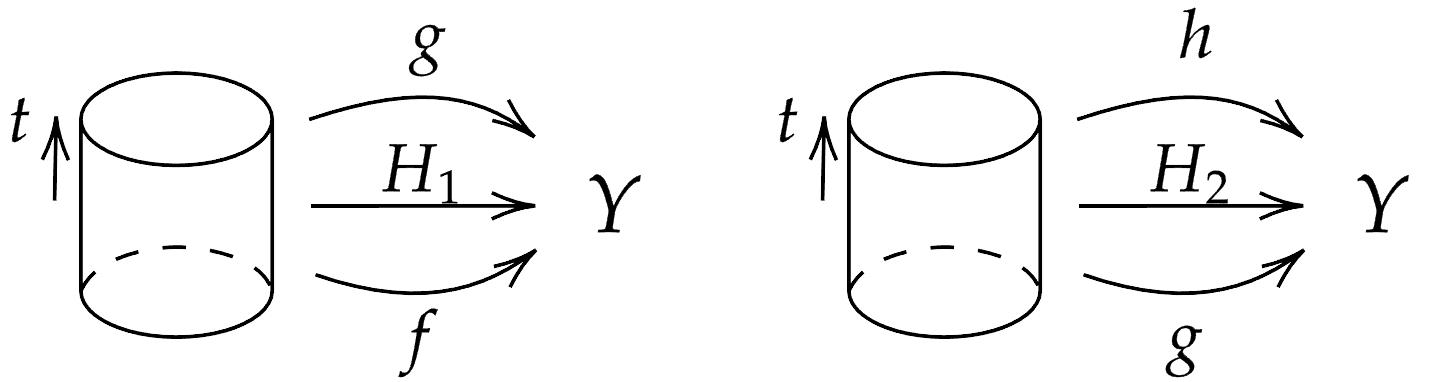
\includegraphics[width=0.6\textwidth]{fig/10.2-1.png}
        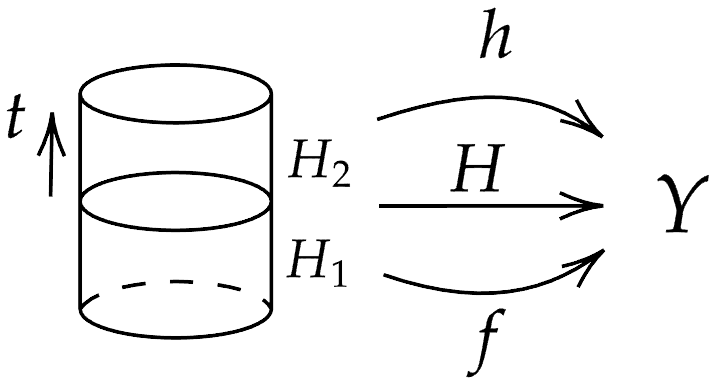
\includegraphics[width=0.3\textwidth]{fig/10.2-2.png}
        \captionof{figure}{同伦的传递性}
    \end{figure}
    
    定义$\setjot[-2]\begin{aligned}[t]
        H:X\times [0,1]&\to Y \\
        (x,t)&\mapsto \begin{cases}
            H_1(x,2t) & 0\leq t\leq \frac{1}{2} \\
            H_2(x,2t-1) & \frac{1}{2}\leq t\leq 1
        \end{cases}
    \end{aligned}$\par
    由粘合引理，$H$是连续的，且$H(x,0)=f(x), H(x,1)=h(x)$. 所以$f\simeq h$.
\end{proof}

\begin{definition}{零同伦}
    如果$f:X\to Y$同伦于常值映射，则称$f$是\textbf{零伦的}.
\end{definition}

\begin{instance}
    $f:X\to \mathbb{E}^n$是零伦的. 事实上，任何映入$\mathbb{E}^n$的凸子空间的映射都是零同伦的.
\end{instance}

\begin{proposition}
    设$f_0\simeq f_1:X\to Y, g_0\simeq g_1:Y\to Z$.
    则$g_0\circ f_0 \simeq g_1\circ f_1:X\to Z$.
\end{proposition}

\begin{proof}
    假设$H_1:f_0\simeq f_1, H_1:X\times [0,1]\to Y$.$H_2:g_0\simeq g_1, H_2:Y\times [0,1]\to Z$.\par
    令$\setjot[-2]\begin{aligned}[t]
        \widetilde{H_1}:X\times [0,1]&\to Y\times [0,1] \\
        (x,t)&\mapsto (H_1(x,t),t)
    \end{aligned}$，则$\widetilde{H_1}$是连续的.\par
    令$H=H_2\circ \widetilde{H_1}:X\times [0,1]\to Z$.
    那么就有$X\times [0,1] \xrightarrow{\widetilde{H_1}} Y\times [0,1] \xrightarrow{H_2} Z$.\par
    $H(x,0)=H_2\circ\widetilde{H_1}(x,0)=H_2(H_1(x,0),0)=H_2(f_0(x),0)=g_0(f_0(x))=g_0\circ f_0(x)$.\par
    $H(x,1)=H_2\circ\widetilde{H_1}(x,1)=H_2(H_1(x,1),1)=H_2(f_1(x),1)=g_1(f_1(x))=g_1\circ f_1(x)$.\par
    所以$g_0\circ f_0 \simeq g_1\circ f_1$.
\end{proof}

\section{相对同伦}

\begin{definition}{相对同伦}
    设$f,g:X\to Y, A\subset X$. 若$f,g$通过$H:X\times [0,1]\to Y$同伦，且$\forall\, a\in A, H(a,t)=f(a)=g(a)$，则称$f$和$g$是\textbf{相对于$A$同伦的}，记作$f\simeq g \text{ rel } A$.
\end{definition}
从定义中可以看出，相对同伦是对同伦概念的加强，它不仅要求普通的同伦，还要求映射在子集$A$上保持不变，即在同伦变换过程中，$A$上的点始终映射到相同的位置.特别地，如果$A=\varnothing$，则相对同伦就是同伦.\par

\begin{remark}
    $\forall\,x\in X, a_x=\setjot[-6]\begin{aligned}[t]
        H(x,\cdot):[0,1] &\to Y \\
        t &\mapsto H(x,t)
    \end{aligned}$是$Y$中的一条道路.\par
    $\forall\,p\in A, a_p=\setjot[-6]\begin{aligned}[t]
        H(p,\cdot):[0,1] &\to Y \\
        t &\mapsto H(p,t)=f(p)=g(p)
    \end{aligned}$是$Y$中的常值道路.
\end{remark}

\begin{instance}
    设$f,g:X\to \mathbb{E}^n, A=\{x\in X\mid f(x)=g(x)\}$.
    构造$\setjot[-2]\begin{aligned}[t]
        H:X\times [0,1]&\to \mathbb{E}^n \\
        (x,t)&\mapsto (1-t)f(x)+tg(x)
    \end{aligned}$\par
    则$\forall\,  a\in A, H(a,t)=(1-t)f(a)+tg(a)=f(a)=g(a)$.
    所以$H:f\simeq g \text{ rel } A$.
\end{instance}

\section{道路同伦}

\begin{definition}{道路同伦}
    设$X$是拓扑空间，$a,b:[0,1]\to X$是两条道路.
    如果$a\simeq b \text{ rel } \{0,1\}$，则称$a$和$b$是\textbf{道路同伦的(定端同伦的)}，记作$a\simeqdot b$.
\end{definition}

具体来说，存在$H:[0,1]\times [0,1]\to X$满足：$H(s,0)=a(s), H(s,1)=b(s)$，$H(0,t)=a(0)=b(0), H(1,t)=a(1)=b(1)$.\par

\begin{figure}[H]
    \centering
    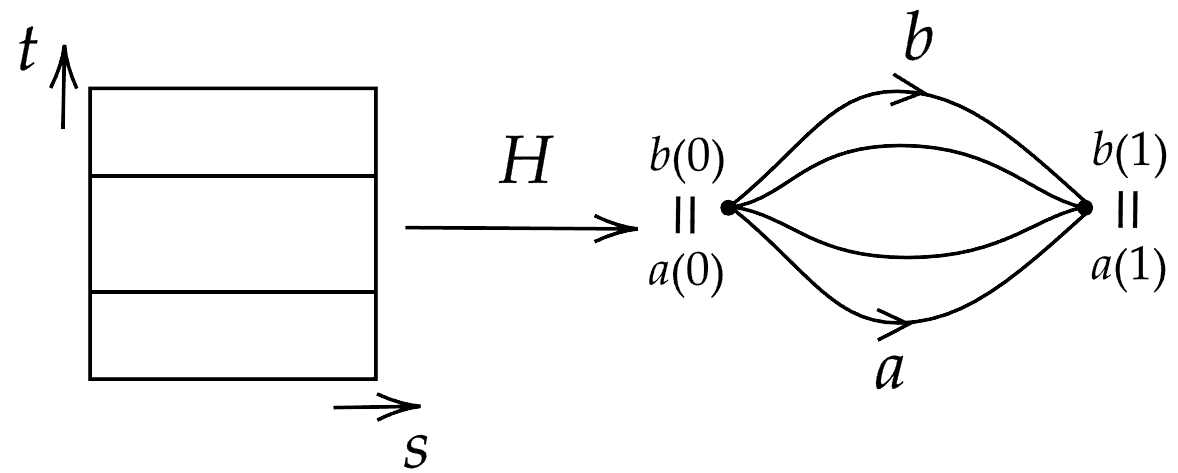
\includegraphics[width=0.6\textwidth]{fig/10.3.png}
    \caption{道路同伦示意图1}
\end{figure}
\vspace{-2 em}
\begin{figure}[H]
    \centering
    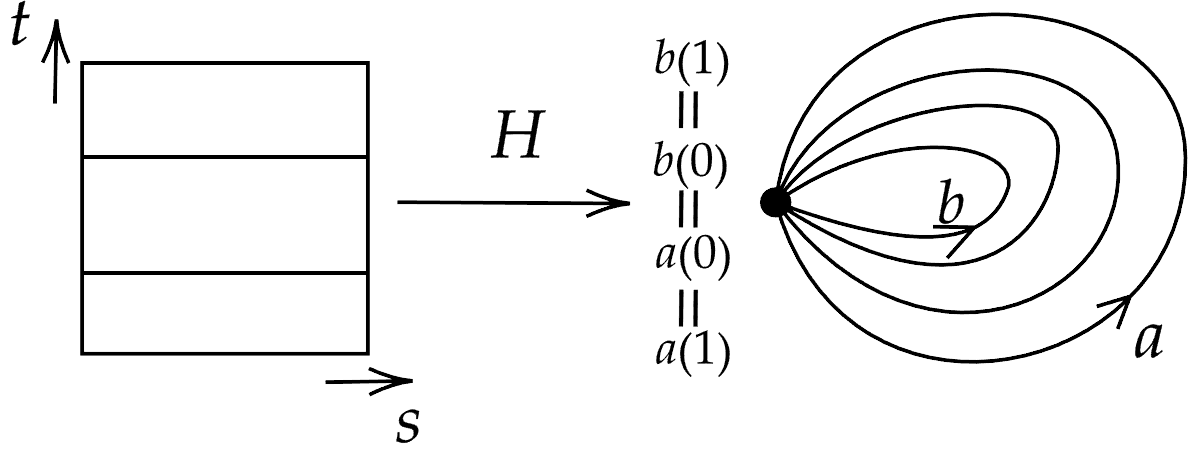
\includegraphics[width=0.6\textwidth]{fig/10.4.png}
    \caption{道路同伦示意图2}
\end{figure}



\begin{definition}{逆道路}
    设$a:[0,1]\to X$是一条道路，定义$a$的\textbf{逆道路}为$ \setjot[-2]\begin{aligned}[t]
    \overline{a}:&[0,1]\to X \\
    t &\mapsto a(1-t)
    \end{aligned}$
\end{definition}

\begin{figure}[H]
    \centering
    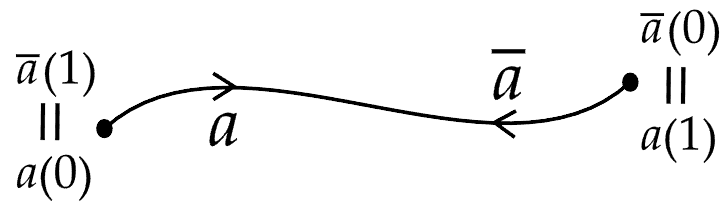
\includegraphics[width=0.4\textwidth]{fig/10.5.png}
    \caption{逆道路示意图}
\end{figure}

\begin{definition}{乘积道路}
    设$a,b:[0,1]\to X$是两条道路，且$a(1)=b(0)$，定义$a$和$b$的\textbf{乘积道路}为\par
    $\setjot[-2]\begin{aligned}[t]
    ab:&[0,1]\to X \\
    t &\mapsto \begin{cases}
            a(2t), & 0\leq t\leq \frac{1}{2} \\
            b(2t-1), & \frac{1}{2}\leq t\leq 1
        \end{cases}
    \end{aligned}$
\end{definition}
\hspace{-2.2em}
\begin{minipage}[t]{0.45\textwidth}
    \vspace{-1 em}
    \begin{figure}[H]
    \centering
    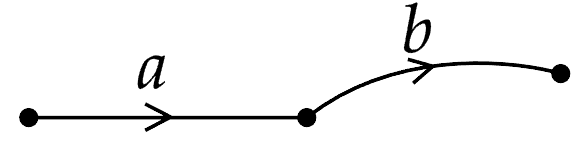
\includegraphics[width=0.7\textwidth]{fig/10.6.png}
    \caption{乘积道路示意图1}
\end{figure}
\end{minipage}
\begin{minipage}[t]{0.45\textwidth}
    \vspace{-2.5 em}
    \begin{figure}[H]
    \centering
    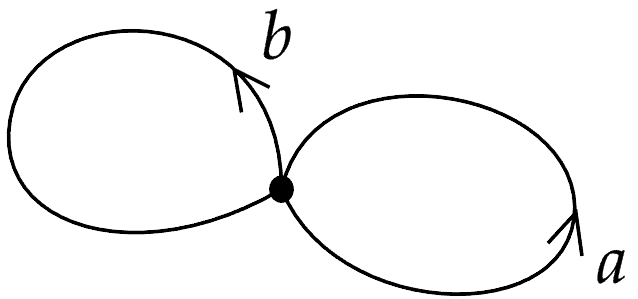
\includegraphics[width=0.6\textwidth]{fig/10.7.png}
    \caption{乘积道路示意图2}
\end{figure}
\end{minipage}


\begin{definition}{道路类}
    道路$a$的\textbf{道路类}定义为$[a]=\{b\mid b\simeqdot a\}$. 如果$a$是一条闭路，则$[a]$称为\textbf{闭路类}，且$a(0)$(或$a(1)$)称为该闭路类的\textbf{基点}.
\end{definition}

\begin{lemma}
    $a\simeqdot b \implies \overline{a}\simeqdot \overline{b}$.
\end{lemma}

\begin{proof}
    假设$H:[0,1]\times [0,1]\to X$实现了$a\simeqdot b$.\par
    令$\setjot[-6]\begin{aligned}[t]
        \overline{H}:[0,1]\times [0,1]&\to X \\
        (s,t)&\mapsto H(1-s,t)
    \end{aligned}$，则$\overline{H}:\overline{a}\simeqdot \overline{b}$.
\end{proof}

\begin{definition}{逆道路类}
    定义道路类$[a]$的\textbf{逆}为$[a]^{-1}:=[ \overline{a} ]$.
\end{definition}

\begin{lemma}
    设$a\simeqdot c, b\simeqdot d$，且$a(1)=b(0)$(从而$c(1)=d(0)$)，则$ab\simeqdot cd$.
\end{lemma}

\begin{proof}
    \begin{figure}[H]
        \centering
        \vspace{-2.8 em}
        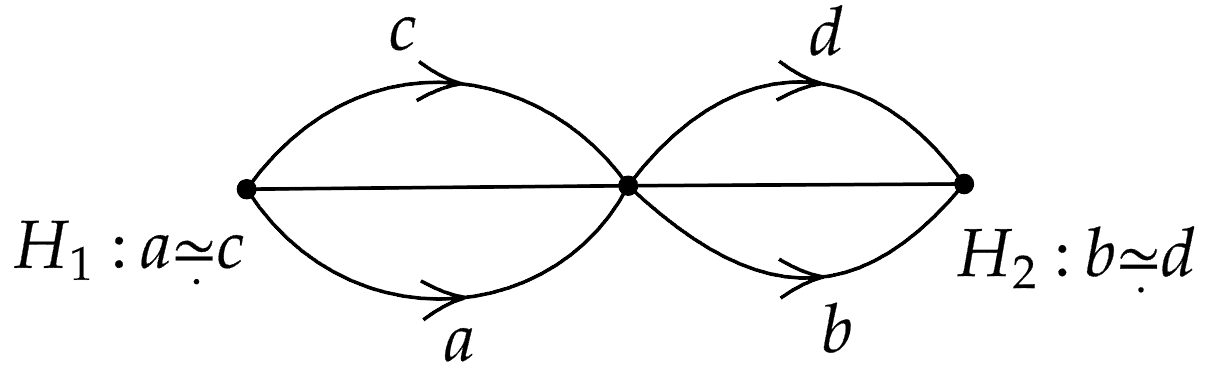
\includegraphics[width=0.5\textwidth]{fig/10.8.png}
        \captionof{figure}{}
    \end{figure}
    \vspace{-1 em}
    设$H_1:a\simeqdot c, H_2:b\simeqdot d$.
    定义$\setjot[-2]\begin{aligned}[t]
        H:[0,1]\times [0,1]&\to X \\
        (s,t)&\mapsto \begin{cases}
            H_1(2s,t), & 0\leq s\leq \frac{1}{2} \\
            H_2(2s-1,t), & \frac{1}{2}\leq s\leq 1
        \end{cases}
    \end{aligned}$\par
    验证边界条件：
    $H(s,0)=\begin{cases}
        H_1(2s,0)=a(2s) &0\leq s\leq\frac{1}{2} \\
        H_2(2s-1,0)=b(2s-1) &\frac{1}{2}\leq s\leq 1
    \end{cases}=(ab)(s)$\par
    类似的，$H(s,1)=(cd)(s)$，且$H(0,t)=a(0)=c(0)$，$H(1,t)=b(1)=d(1)$.\par
    由粘合引理，$H$是连续的. 所以$ab\simeqdot cd$.
\end{proof}

\begin{definition}{道路类的乘积}
    设$[a],[b]$是两个道路类，且$a(1)=b(0)$，定义它们的\textbf{乘积}为$[a]\cdot [b]:=[ab]$.
\end{definition}

\section{基本群}

\vspace{-1 em}
\begin{definition}{基本群}
    设$X$是拓扑空间，$x_0\in X$.
    定义$\pi_1(X,x_0)=\{ \text{所有以}\,x_0\,\text{为基点的闭路类} \}$.
    对于任意两个闭路类$[a],[b]\in \pi_1(X,x_0)$，定义运算$[a]\cdot [b]=[ab]\in \pi_1(X,x_0)$.
\end{definition}
\begin{figure}[H]
    \vspace{-1 em}
    \centering
    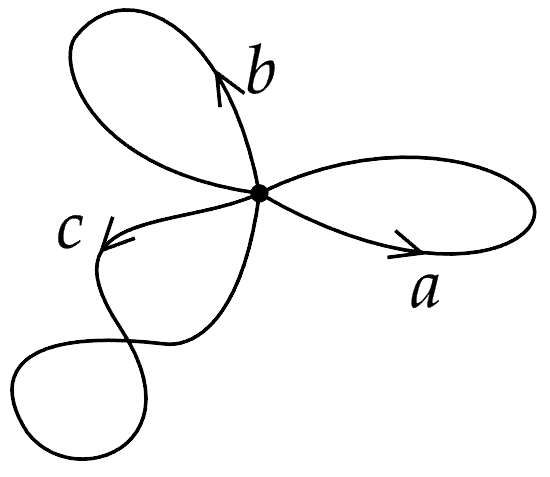
\includegraphics[width=0.3\textwidth]{fig/10.9.png}
    \captionof{figure}{}
\end{figure}

\begin{lemma}[运算的结合律]
    设$a,b,c:[0,1]\to X$是道路，且$a(1)=b(0), b(1)=c(0)$，则$\left([a]\cdot [b]\right)\cdot [c] = [a]\cdot \left([b]\cdot [c]\right)$.
    特别地，$\pi_1(X,x_0)$中的乘法满足\textbf{结合律}.
\end{lemma}

\begin{proof}
    $([a]\cdot [b])\cdot [c] = [ab]\cdot [c] = [(ab)c]$.
    $[a]\cdot ([b]\cdot [c]) = [a]\cdot [bc] = [a(bc)]$.
    只需证明$(ab)c \simeqdot a(bc)$.
    则\[((ab)c)(s)=\begin{cases}
            a(4s), & 0\leq s\leq \frac{1}{4} \\[5pt]
            b(4s-1), & \frac{1}{4}\leq s\leq \frac{1}{2} \\[5pt]
            c(2s-1), & \frac{1}{2}\leq s\leq 1
        \end{cases}\quad\quad
        (a(bc))(s) = \begin{cases}
            a(2s), & 0\leq s\leq \frac{1}{2} \\[5pt]
            b(4s-2), & \frac{1}{2}\leq s\leq \frac{3}{4} \\[5pt]
            c(4s-3), & \frac{3}{4}\leq s\leq 1
        \end{cases}\]\par
    \begin{figure}[H]
        \centering
        \vspace{-1 em}
        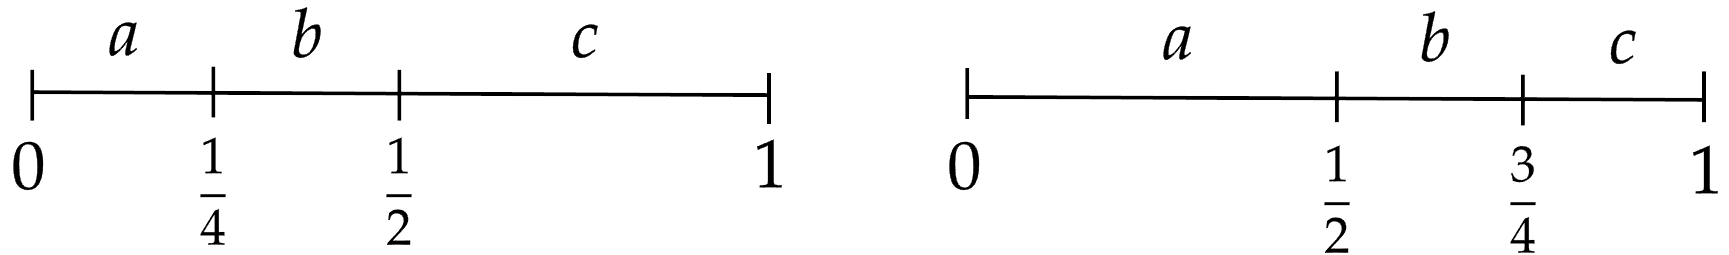
\includegraphics[width=0.65\textwidth]{fig/10.10.png}
        \captionof{figure}{}
    \end{figure}
    \begin{wrapfigure}{r}{0.28\textwidth}
        \vspace{-2  em}
        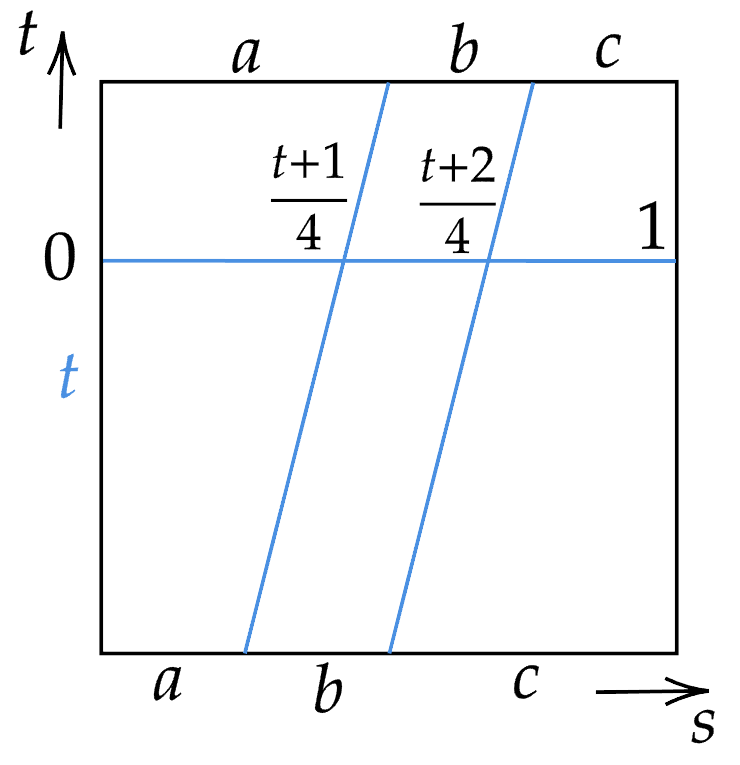
\includegraphics[width=0.28\textwidth]{fig/10.11.png}
        \captionof{figure}{}
        \vspace{-1 em}
    \end{wrapfigure}
    \vspace{-1 em}
    令$\setjot[-2]\begin{aligned}[t]
        H:[0,1]\times [0,1]&\to X \\
        (s,t)&\mapsto \begin{cases}
            a\left(\frac{4s}{t+1}\right), & 0\leq s\leq \frac{t+1}{4} \\
            b\left(4s-t-1\right), & \frac{t+1}{4}\leq s\leq \frac{t+2}{4} \\
            c\left(\frac{4s-t-2}{2-t}\right), & \frac{t+2}{4}\leq s\leq 1
        \end{cases}
    \end{aligned}$\par
    则$H(s,0)=(ab)c(s),H(s,1)=a(bc)(s)$\par
    $H(0,t)=a(0),H(1,t)=c(1)$.\par
    由粘贴引理，$H$连续，故$H:(ab)c \simeqdot a(bc)$.
\end{proof}

\begin{lemma}
    设$a:[0,1]\to X, a(0)=x_0, a(1)=x_1$，则$[c_{x_0}]\cdot [a] = [a] = [a]\cdot [c_{x_1}]$，其中$c_{x_0}, c_{x_1}$是常值道路.
    特别地，$[c_{x_0}]$是$\pi_1(X,x_0)$中的\textbf{单位元}.
\end{lemma}

\begin{proof}
    只需证明$c_{x_0}\cdot a \simeqdot a \simeqdot a\cdot c_{x_1}$.\par
    \begin{wrapfigure}{r}{0.22\textwidth}
        \vspace{-3  em}
        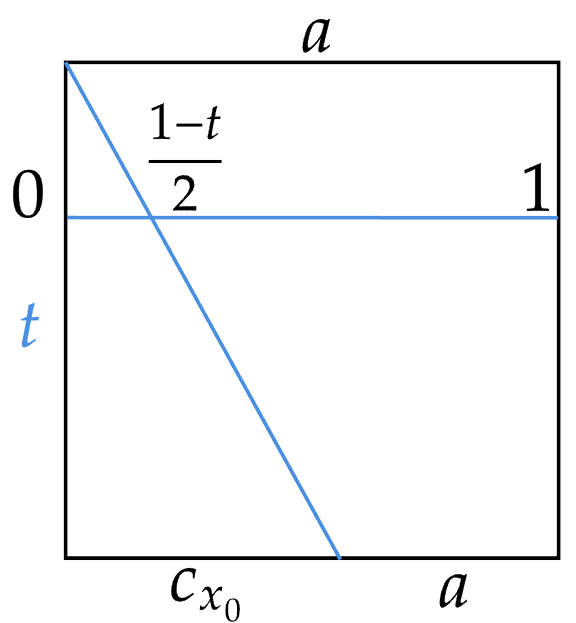
\includegraphics[width=0.22\textwidth]{fig/10.12.png}
        \captionof{figure}{}\par
        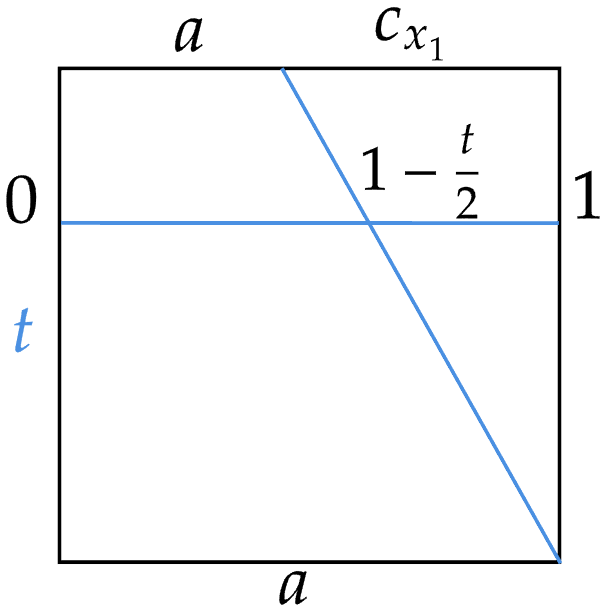
\includegraphics[width=0.22\textwidth]{fig/10.13.png}
        \captionof{figure}{}
        \vspace{-1 em}
    \end{wrapfigure}
    构造$\setjot[-2]\begin{aligned}[t]
        H_1:[0,1]\times [0,1]&\to X \\
        s,t &\mapsto \begin{cases}
            x_0, & 0\leq s\leq \frac{1-t}{2} \\
            a\left(\frac{2s+t-1}{t+1}\right), & \frac{1-t}{2}\leq s\leq 1
        \end{cases}
    \end{aligned} $\par
    则$H_1$连续，且$H_1:c_{x_0}\cdot a \simeqdot a$.\par
    同理可构造$\setjot[-2]\begin{aligned}[t]
        H_2:[0,1]\times [0,1]&\to X \\
        (s,t) &\mapsto  \begin{cases}
            a\left(\frac{2s}{2-t}\right), & 0\leq s\leq 1-\frac{t}{2} \\
            x_1, & \frac{1-t}{2}\leq s\leq 1
        \end{cases}
    \end{aligned} $\par
    则$H_2$连续，且$H_2:a \simeqdot a\cdot c_{x_1}$
    \vspace{4 em}
\end{proof}

\begin{lemma}
    设$a:[0,1]\to X, a(0)=x_0, a(1)=x_1$，则$[a]\cdot [a]^{-1} = [c_{x_0}], [a]^{-1}\cdot [a] = [c_{x_1}]$.
    特别地，$\pi_1(X,x_0)$中的任意闭路类都有\textbf{逆元}.
\end{lemma}

\begin{proof}
    只需证明$a\cdot \overline{a} \simeqdot c_{x_0}$(与$\overline{a}\cdot a\simeqdot c_{x_1}$等价).
    \begin{figure}[H]
        \centering
        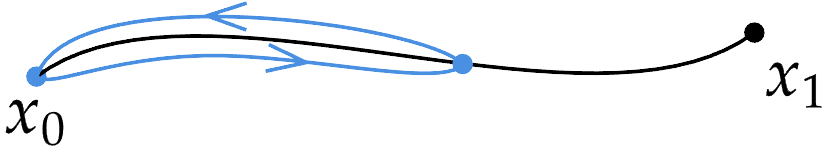
\includegraphics[width=0.35\textwidth]{fig/10.14.png}
        \captionof{figure}{}
    \end{figure}
    \begin{wrapfigure}{r}{0.22\textwidth}
        \vspace{-3  em}
        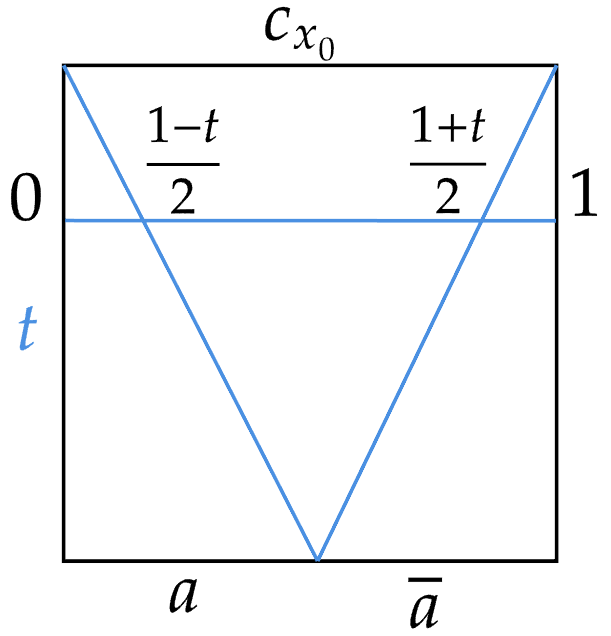
\includegraphics[width=0.22\textwidth]{fig/10.15.png}
        \captionof{figure}{}
    \end{wrapfigure}
    构造$\setjot[-2]\begin{aligned}[t]
        H:[0,1]\times [0,1]&\to X \\
        (s,t) &\mapsto \begin{cases}
            a(2s), & 0\leq s\leq \frac{1-t}{2} \\[3pt]
            a(1-t), & \frac{1-t}{2}\leq s\leq \frac{1+t}{2} \\[3pt]
            \overline{a}(2s-1), & \frac{1+t}{2}\leq s\leq 1
        \end{cases}
    \end{aligned} $ \par
    \bluebf{整个过程可以描述为：$a(0)\to a(1-t)=\overline{a(t)}\to \overline{a}(1)$}\par
    则$H:a\overline{a}\simeqdot c_{x_0}$
\end{proof}

\begin{theorem}
    $\pi_1(X,x_0)$是一个群，称为$X$的以$x_0$为基点的\textbf{基本群}.
\end{theorem}

\begin{instance}
    $\pi_1(\mathbb{E}^n, x_0) = \{1\}$，平凡群.
    因为对于任意闭路$a$，都有$a\simeqdot c_{x_0}$（通过直线同伦）.
\end{instance}

\begin{instance}
    如果$X$是$\mathbb{E}^n$的凸子空间，则$\pi_1(X,x_0)=\{1\}$.
\end{instance}

\section{诱导同态}

\begin{definition}{同态}
    设$G_1, G_2$是两个群，若$\varphi:G_1\to G_2$满足$\varphi(gh)=\varphi(g)\varphi(h)$，则称$\varphi$是\textbf{同态}.
\end{definition}
因此，同态保持了群的运算结构.


\begin{instance}
    $\setjot[-8]\begin{aligned}[t]
        \varphi:\mathbb{Z}&\to \mathbb{Z} \\
        z &\mapsto 2z
    \end{aligned}$，$\setjot[-8]\begin{aligned}[t]
        \varphi:\mathbb{Z}&\to \mathbb{Z} \\
        z &\mapsto z+1
    \end{aligned}$，$\setjot[-8]\begin{aligned}[t]
        \varphi_2:\mathbb{Z}&\to \mathbb{Z} \\
        z&\mapsto 0
    \end{aligned}$，上述三个均为同态，其中第三个称为\bluebf{平凡同态}
\end{instance}

设$X,Y$是两个空间，$f:X\to Y$是连续映射.
$a:[0,1]\to X$是$X$中的道路，则$f\circ a:[0,1]\to Y$是$Y$中的道路.

\begin{lemma}
    若在$X$中$a\simeqdot b$，则在$Y$中$f\circ a \simeqdot f\circ b$.
\end{lemma}

\begin{proof}
    假设$H:a\simeqdot b$.
    $H:[0,1]\times [0,1]\to X$.
    \begin{figure}[H]
        \centering
        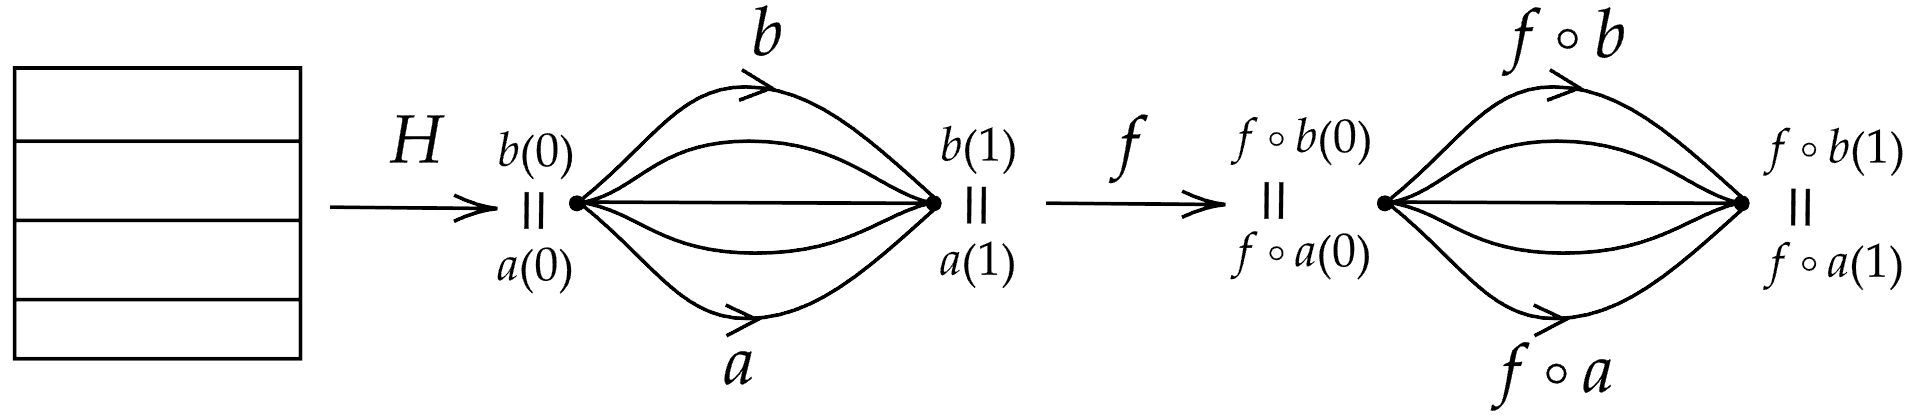
\includegraphics[width=0.8\textwidth]{fig/10.16.png}
        \captionof{figure}{}
    \end{figure}
    $f\circ H:[0,1]\times [0,1]\to Y$.
    则$f\circ H: f\circ a \simeqdot f\circ b$.
\end{proof}

\begin{definition}
    $f:X\to Y$诱导了一个映射$\setjot[-2]\begin{aligned}[t]
            f_*:\pi_1(X,x_0) &\to \pi_1(Y,f(x_0)) \\
            [a] &\mapsto [f\circ a]
        \end{aligned}$.
\end{definition}

\begin{lemma}
    $f_*$是一个同态.
\end{lemma}

\begin{proof}
    设$[a],[b]\in \pi_1(X,x_0)$.$\setjot[-2]\begin{aligned}[t]
        f_*([a]\cdot [b]) &= f_*([a\cdot b]) = [f\circ (a\cdot b)]=[(f\circ a)\cdot (f\circ b)] \\
        & = [f\circ a]\cdot [f\circ b] = f_*[a]\cdot f_*[b].
    \end{aligned}$
    \begin{figure}[H]
        \centering
        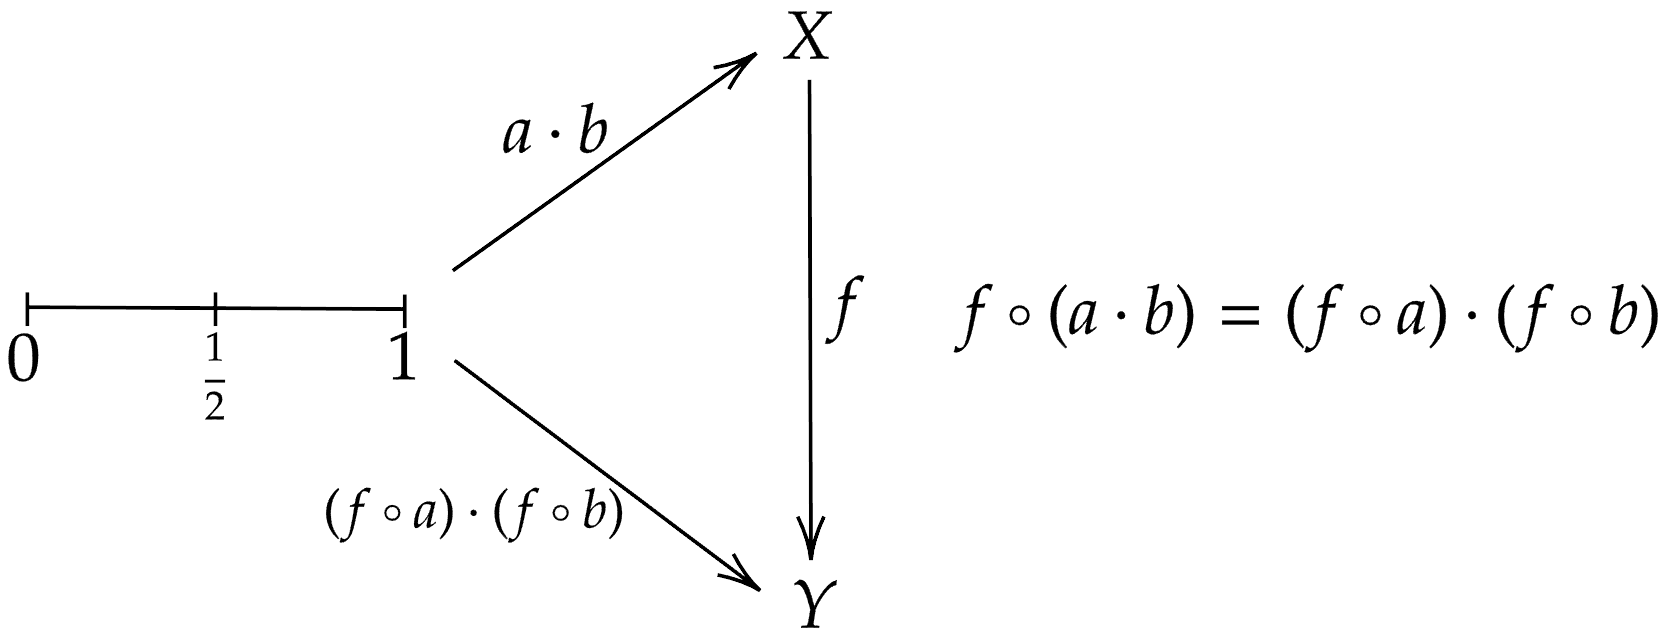
\includegraphics[width=0.6\textwidth]{fig/10.17.png}
        \captionof{figure}{证明图例}
    \end{figure}
\end{proof}

\begin{instance}
    $\setjot[-8]\begin{aligned}[t]
        f:X&\to Y \\
        x &\mapsto y_0
    \end{aligned}$是常值映射，则$\setjot[-4]\begin{aligned}[t]
            f_*:\pi_1(X,x_0) &\to \pi_1(Y,y_0) \\
            [a] &\mapsto [f\circ a] = [c_{y_0}]
        \end{aligned}$是平凡同态.
\end{instance}

\begin{instance}
    $\setjot[-8]\begin{aligned}[t]
        \mathrm{id}:X&\to X \\
        x &\mapsto x
    \end{aligned}$，则$\setjot[-4]\begin{aligned}[t]
            (\mathrm{id})_*:\pi_1(X,x_0) &\to \pi_1(X,x_0) \\
            [a] &\mapsto [a]
        \end{aligned}$是恒等同构.
\end{instance}

\begin{lemma}
    设$f:X\to Y, g:Y\to Z, x_0\in X$.
    则$(g\circ f)_* = g_*\circ f_*: \pi_1(X,x_0)\to \pi_1(Z,g(f(x_0)))$.
\end{lemma}

\begin{proof}
    $\forall [a]\in \pi_1(X,x_0), (g\circ f)_*([a]) = [g\circ f\circ a]$
    $= g_*[f\circ a] = g_*(f_*[a]) = g_*\circ f_*[a]$.
\end{proof}

\begin{theorem}
    设$f:X\to Y$是同胚，$x_0\in X$.
    则$f_*:\pi_1(X,x_0)\to \pi_1(Y,f(x_0))$是一个同构.
\end{theorem}

\begin{proof}
    设$f^{-1}:Y\to X$是$f$的逆映射.
    $f^{-1}\circ f = id_X: X\to X$. $f\circ f^{-1} = id_Y: Y\to Y$.
    \[
        (f^{-1})_*\circ f_* = (f^{-1}\circ f)_* = (id_X)_*: \pi_1(X,x_0)\to \pi_1(X,x_0)
    \]
    \[
        \pi_1(X,x_0) \xrightarrow{f_*} \pi_1(Y,f(x_0)) \xrightarrow{(f^{-1})_*} \pi_1(X,x_0)
    \]
    复合映射是恒等映射.
    则$f_*$是单射，$(f^{-1})_*$是满射.
    \[
        f_*\circ (f^{-1})_* = (f\circ f^{-1})_* = (id_Y)_*: \pi_1(Y,f(x_0))\to \pi_1(Y,f(x_0))
    \]
    \[
        \pi_1(Y,f(x_0)) \xrightarrow{(f^{-1})_*} \pi_1(X,x_0) \xrightarrow{f_*} \pi_1(Y,f(x_0))
    \]
    复合映射是恒等映射.
    则$(f^{-1})_*$是单射，$f_*$是满射.
    所以$f_*$是一个同构.
\end{proof}

\section{基点的移动}

设$X$是道路连通空间，$x_0,x_1\in X$.
$w$是从$x_0$到$x_1$的道路类.
\begin{figure}[H]
    \centering
    \includegraphics[width=0.6\textwidth]{example-image}
    \caption{基点移动示意图}
\end{figure}
$\forall \alpha \in \pi_1(X,x_0)$，则$w^{-1}\alpha w \in \pi_1(X,x_1)$.
定义
\[
    \begin{aligned}
        w_\#:\pi_1(X,x_0) &\to \pi_1(X,x_1) \\
        \alpha &\mapsto w^{-1}\alpha w
    \end{aligned}
\]

\begin{lemma}
    $w_\#$是一个同态.
\end{lemma}

\begin{proof}
    设$\alpha,\beta \in \pi_1(X,x_0)$. 注意$w\cdot w^{-1} \simeqdot c_{x_0}$.
    \[
        w_\#(\alpha\cdot \beta) = w^{-1}\alpha\beta w \simeqdot w^{-1}\alpha w w^{-1}\beta w
    \]
    \[
        = w_\#(\alpha)\cdot w_\#(\beta).
    \]
\end{proof}

\begin{instance}
    设$w=[c_{x_0}]$.
    \[
        \begin{aligned}
            [c_{x_0}]_\#:\pi_1(X,x_0) &\to \pi_1(X,x_0) \\
            \alpha &\mapsto [c_{x_0}]^{-1}\cdot \alpha \cdot [c_{x_0}] = \alpha
        \end{aligned}
    \]
    是恒等映射$id$.
\end{instance}

\begin{figure}[H]
    \centering
    \includegraphics[width=0.6\textwidth]{example-image}
    \caption{道路复合示意图}
\end{figure}

\begin{lemma}
    设$w'$是从$x_1$到$x_2$的道路类.
    $(w\cdot w')_\#:\pi_1(X,x_0)\to \pi_1(X,x_2)$.
    则$(w\cdot w')_\# = (w')_\# \circ w_\#$.
\end{lemma}

\begin{proof}
    $\forall \alpha \in \pi_1(X,x_0)$.
    \[
        (ww')_\#(\alpha) = (ww')^{-1}\cdot \alpha \cdot ww'
    \]
    \[
        = (w')^{-1}\cdot w^{-1}\alpha \cdot w \cdot w' = (w')^{-1}\cdot w_\#(\alpha) \cdot w'
    \]
    \[
        = (w')_\#(w_\#(\alpha)) = (w')_\# \circ w_\#(\alpha).
    \]
\end{proof}

\begin{proposition}
    $w_\#:\pi_1(X,x_0)\to \pi_1(X,x_1)$是一个同构.
\end{proposition}

\begin{proof}
    \begin{figure}[H]
        \centering
        \includegraphics[width=0.6\textwidth]{example-image}
        \caption{同构证明示意图}
    \end{figure}
    $w\cdot w^{-1} \simeqdot c_{x_0}$，$w^{-1}\cdot w \simeqdot c_{x_1}$.
    由上述引理，
    \[
        (w^{-1}\cdot w)_\# = w_\# \circ (w^{-1})_\# : \pi_1(X,x_1)\to \pi_1(X,x_1)
    \]
    是恒等映射$id$.
    \[
        \pi_1(X,x_1) \xrightarrow{(w^{-1})_\#} \pi_1(X,x_0) \xrightarrow{w_\#} \pi_1(X,x_1)
    \]
    复合映射是$id$.
    则$w_\#$是满射.
    
    \[
        (w\cdot w^{-1})_\# = (w^{-1})_\# \circ w_\# : \pi_1(X,x_0)\to \pi_1(X,x_0)
    \]
    是恒等映射$id$.
    \[
        \pi_1(X,x_0) \xrightarrow{w_\#} \pi_1(X,x_1) \xrightarrow{(w^{-1})_\#} \pi_1(X,x_0)
    \]
    复合映射是$id$.
    则$w_\#$是单射.
    所以$w_\#$是一个同构.
\end{proof}

\begin{corollary}
    设$X$是道路连通空间，$x_0,x_1\in X$.
    则$\pi_1(X,x_0)\cong \pi_1(X,x_1)$.
\end{corollary}

\begin{remark}
    $\pi_1(X,x_0)\cong \pi_1(A,x_0)$，其中$A$是$X$中包含$x_0$的道路连通分支.
    \begin{figure}[H]
        \centering
        \includegraphics[width=0.6\textwidth]{example-image}
        \caption{道路连通分支示意图}
    \end{figure}
    如果$X$是道路连通的，则有时$\pi_1(X,x_0)$简写为$\pi_1(X)$.
    $\pi_0(X)$是$X$的道路连通分支的集合.
\end{remark}

\begin{definition}{单连通}
    设$X$是道路连通的. 如果$\pi_1(X,x_0)=\{1\}$，则称$X$是\textbf{单连通的}(simply connected).
\end{definition}



